\chapter{Background}

\section{Representing Geometry}
\subsection{Triangles}
To develop an interactive 3D application a scene representation is needed. Traditionally, all geometric objects in a scene are represented by triangles. For example, to model a simple cube we can represent each of its faces using two triangles for a total of 12 triangles. The reason for using triangles is due to their geometric simplicity (triangles contain the fewest number of points that define a plane). Also, as dedicated Graphics Processing Units (GPUs) became more common they were designed with this traditional triangle rasterization in mind so they have specialized hardware to operate on triangles. In other words, triangles are fast to process.

But triangles do have some issues. Primarily, they do a good job of representing surfaces (since they are inherently 2D) but they don't lend themselves well to volumetric (3D) data. For example, a natural representation of a cloud would be a 3D volume filled with the density of the cloud at a given point within the volume. There are algorithms that can convert from a volumetric representation to a triangle one---marching cubes~\cite{lorensen1987marching} being the most popular---but it still only models an arbitrary isosurface as opposed to the actual volume.

\subsection{Voxels}
Voxels (volume elements) represent 3D objects in a natural way. A volumetric representation of an object is a 3D grid of cells (the voxels) which hold any data relevant to that voxel: color, transparency, and normal, to name a few. Recently, voxels have grown popular in the computer graphics field due to this natural representation of 3D objects. The main reason voxels were not used much in the past is due to the amount of memory required to store a voxelized representation as well as GPUs being specialized for triangle rasterization. This restriction has largely been lifted since modern GPUs have much more memory and general purpose GPU (GPGPU) computing has allowed programmers to work more easily with non-triangle based computing.

\begin{figure}[h]
\centering
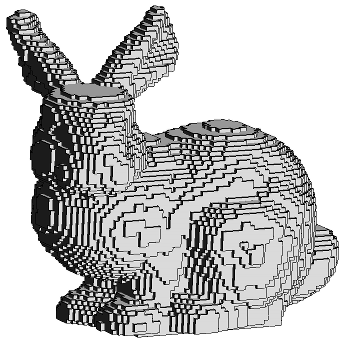
\includegraphics[scale=0.5]{bunny_voxel.png}
\caption{Voxelized representation of a bunny (image from \url{http://cse.iitkgp.ac.in/\textasciitilde pb}).}
\label{fig:bunnyvoxel}
\end{figure}

\section{Computer Graphics Primer}
This thesis has a heavy focus on implementation details and requires a solid foundation in understanding computer graphics. Thus this brief primer will introduce the most important topics including the graphics pipeline, transforms, and some common graphics terminology and techniques.

\subsection{The Graphics Pipeline and Rasterization}
The ultimate goal of most graphics work is to produce a 2D image from some set of input data, typically a scene filled with triangle meshes and various light sources. This process is accomplished in several distinct stages which compose the classic graphics pipeline, some of which are configurable through shaders. We give a brief overview of the pipeline here, but encourage referring to TODO for a more detailed explanation.

The input to the pipeline is a series of vertices. Each vertex contains associated information such as its position in 3D space, a surface normal, and a texture coordinate.

The first step in the pipeline is \textbf{vertex shading}, where a vertex shader is executed for each input vertex. Most vertex shaders are fairly simple and perform the job of transforming the input vertex's position from one coordinate system to another.

After vertex shading, \textbf{shape assembly} occurs and forms geometric primitives from the vertices. The most common primitive is the triangle, although other options such as points and lines exist.

Optionally, \textbf{geometry shading} can take place to operate on the primitives generated from shape assembly. Some common uses here are to introduce more primitives into the pipeline or to modify the input primitive before proceeding to rasterization.

\textbf{Rasterization} involves generating fragments for each primitive that will end up on the screen~\footnote{The primitives go through clipping immediately before rasterization, which removes fragments outside the screen}. Each fragment corresponds to one pixel in the final rendered image and is generated by testing whether a given pixel is contained within an input primitive. The resolution of the fragments is determined by the viewport resolution, which is generally set to the resolution of the framebuffer being rendered to.

During \textbf{fragment shading}, a fragment shader is executed for each fragment generated during rasterization. The output of this shader is typically the color of the pixel for the final image, which is written into a framebuffer. This stage is also where the majority of shading effects occur, including lighting.

Finally, each shaded fragment goes through a \textbf{testing and blending} phase. Depth testing is used to determine whether one fragment is in front of or behind the value currently in the framebuffer. Alpha testing and blending occurs when the fragment is transparent (the alpha, or opacity, value is less than one). The tests and blending can be configured and enabled/disabled as desired (but is not performed programmatically in a shader).

\subsection{Transforms}
A crucial part of computer graphics is transforming points from one coordinate system to another. Transformations are needed to ensure objects are placed correctly in the virtual world and then to project them from 3D space into a 2D space that can be rasterized and displayed on the screen. Most transformations are represented as matrices so that applying a transformation to a vector is just multiplication. Note that OpenGL uses a right-handed coordinate system: if the coordinate system is aligned with our screen then the $x$ axis points right, $y$ points up, and $z$ points \textit{out of} the screen (the `forward' direction is $-z$).

Some important coordinate systems for computer graphics and this work are:
\begin{description}
    \item[Object Space:] the local coordinate system for an object. This is the initial space all vertex coordinates are in when loaded from a mesh.
    \item[World Space:] the global coordinate system for the virtual world. Objects are placed into the world using a \textbf{model} matrix.
    \item[View Space:] the virtual world given from the perspective of a camera (the viewer). The camera is centered at $(0,0,0)$ and faces in the $-z$ direction. The transformation from world space to view space is accomplished using a \textbf{view} matrix.
    \item[Clip Space:] a coordinate system `clipped' to the range $[0, 1]$. Sometimes also referred to as being in Normalized Device Coordinates (NDC), the $z$ axis is also `flipped' compared to the standard OpenGL right-handed coordinate system. A \textbf{projection} matrix is used to transform from view space to clip space, of which there are two general kinds: perspective, which emulates how objects further away from a camera appear smaller, and orthographic, which preserves size regardless of distance from camera.
    \item[Screen Space:] the coordinate space representing a typical 2D screen or image. The $x$ and $y$ coordinates are the respective pixel position (treating the bottom left corner as $(0,0)$). The $z$ axis is usually interpreted as the depth of the pixel as a value within the range $[0, 1]$. The conversion from clip space to screen space is done automatically by the GPU during rasterization based on the viewport resolution.
    \item[Texture Space:] the coordinate space used when sampling a value from a texture. The coordinates are within the range $[0, 1]$, with $(0, 0)$ being the bottom left corner. Sampling outside this range results in behavior defined by a textures wrapping mode (e.g.\ clamp to the edge value or repeat the texture).
    \item[Image Space:] the coordinate space used when indexing into an image. The range is defined by the target image and uses integral numbers.
    \item[Light Space:] similar to the view space, but instead of the camera defining the origin and orientation a light source is used.
    \item[Tangent Space:] a coordinate system defined with respect to a surface and its normal.
\end{description}

\subsection{Compute Shaders}
While most graphics work follows the graphics pipeline, it is possible to use a more abstract model suited towards general purpose computing. Compute shaders provide an interface to performing this GPGPU work (similar to how CUDA exposes GPGPU oepration). At the most basic level, dispatching a compute shader launches many threads that all execute the same program, or kernel, defined in the shader. The inputs and outputs of a compute shader are completely user-defined. More information on compute shaders and GPGPU can be found at TODO.

\subsection{Textures and Mipmapping}
A texture in the most basic sense is a linear buffer of data. In computer graphics, the most common texture is a 2D texture storing color and opacity values, requiring four components---three for the RGB color and one for the opacity. However, 1D and 3D textures are also possible (and 3D textures are a core part of this thesis) as well as various data formats. Textures can also contain multiple levels, often used for mipmapping. OpenGL and GPUs have native support for working with multi-level textures and sampling from them appropriately.

Typically, textures can be considered read-only: they are only sampled from inside a shader. To write to a texture, there are two common approaches: render-to-texture and binding the texture as an image (a type of object in OpenGL). Render-to-texture refers to attaching the texture to a framebuffer object, which can then be used as the target for rasterization. The other method involves binding a single level of a texture as an image object which can then be written to inside a shader (usually a fragment or compute shader).

% TODO should explain why it smooths
% TODO move before previous paragraph?
Mipmapping involves keeping multiple detail levels of the same source data. The base level is the highest resolution available and each successive level is downscaled. While this does require increased memory usage, it can smooth out aliasing issues caused by sampling. Mipmapping also generally increases performance as it improves GPU texture cache locality.

% TODO section on basic graphics stuff like mipmapping, shadow mapping, normal mapping, transforms?

% opengl datatypes and formats? texture formats + levels might help

\section{Spatial Data Structures}
Many algorithms in computer graphics require a way to query particular aspects about a particular point or object in space. These queries could be something like ``which side of a plane is this object on'' or, more relevant to our work, ``how much light is present at this point''. Of course, this data could be stored in a simple array but oftentimes this leads to poor runtime performance. Using a more advanced data structure to represent spatial data is crucial to achieving real-time rendering performance. We briefly describe some common data structures relevant to our work.

\subsection{3D Textures}
One of the simplest approaches to storing spatial data is to simply define a uniform mapping from 3D space into a 3D texture, essentially a cube. While this is straightforward to visualize and is easy to work with, 3D textures require a large amount of memory. If the data to be stored is sparse (i.e.\ most positions in space do not have a corresponding value) this memory is wasted. Also, GPUs are able to take advantage of spatial coherency in 3D textures and can provide fast caching and filtering of the data.

\subsection{Clipmaps}
In a 3D texture, we essentially have a uniform grid of values: the resolution, or level of detail, of data remains constant throughout the entire texture. With many types of data, we don't need the same resolution---for example, in many applications, the farther away from the viewer we are the less detail we need. A clipmap~\cite{Tanner:1998:CVM:280814.280855, Losasso:2004:GCT:1186562.1015799} is based on this concept and represents 3D space using differing levels of detail. The resolution at each level of detail is halved, reducing the amount of memory needed to represent the same 3D space as an equivalent 3D texture. The issue with sparse memory still exists, but it is alleviated greatly.

\begin{figure}[h]
\centering
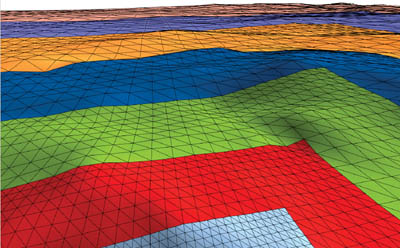
\includegraphics[scale=1.0]{geometry_clipmap.jpg}
\caption{Example of clipmaps applied to terrain. Notice that the inner levels have higher detail while each successive outer level lowers the detail level by a factor of 2 (image from~\cite{Losasso:2004:GCT:1186562.1015799}).}
\label{fig:geometryclipmaps}
\end{figure}

\subsection{Octrees}
Another way of representing 3D space can be done using a tree structure. An octree~\cite{Cra12, meagher1982geometric} is a tree where each child node is an octant of its parent (see Figure~\ref{fig:octree}). This representation is very efficient memory wise when it comes to sparse data since there is no requirement the tree has to be full: if there is no data in an octant, we can leave it childless. The tradeoff, however, is we have to recurse through the octree for every query. This can be difficult to do on the GPU and it loses the hardware supported caching and filtering provided to 3D textures.

\begin{figure}[h]
\centering
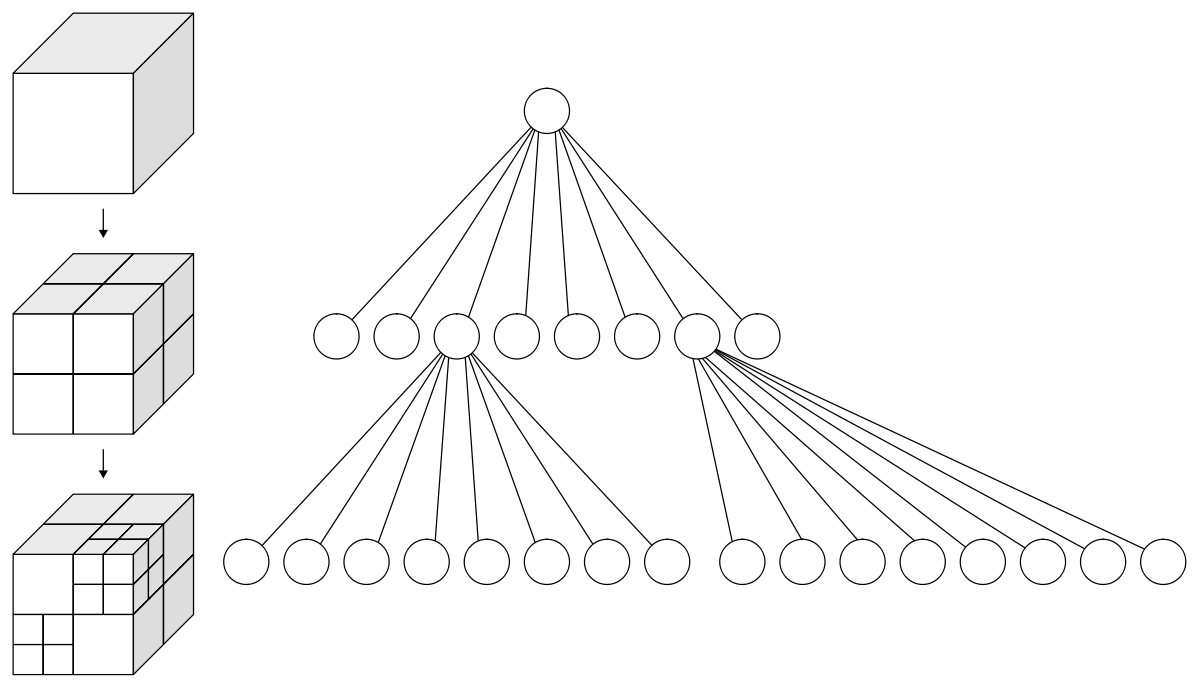
\includegraphics[scale=0.25]{octree.png}
\caption{Diagram of a simple octree (image from \url{https://en.wikipedia.org/wiki/Octree}).}
\label{fig:octree}
\end{figure}

\section{Radiance and the Rendering Equation}
As our goal is to accurately model light in our virtual scene, it makes sense to base our shading model on the behavior of real light. The theoretical basis for understanding and measuring light is confined within the field of radiometry. Fortunately, for our purposes, we can focus more on the applied aspects of radiometry for computer graphics---for example, the wave-like nature of light is mostly ignored in favor of particle based behavior.

Fundamentally, light is energy. Therefore, our goal is to compute the amount of light energy at a surface point from a given viewpoint (our camera). This quantity, called radiance, is the instantaneous amount of light energy emitted along the ray of light from the point to the camera. Kajiya~\cite{kajiya1986rendering} presents this problem mathematically in the rendering equation:
\begin{equation*}
    L_o(\bm{x}, \omega_o) = L_e(\bm{x}, \omega_o) + \int_\Omega f_r(\bm{x}, \omega_i, \omega_o)\ L_i(\bm{x}, \omega_i)\ (\omega_i \cdot \bm{n})\ d\omega_i
\end{equation*}
where
\begin{description}
    \item[$\bm{x}$] is a point in space,
    \item[$\omega_o$] is the direction of outgoing light from $\bm{x}$,
    \item[$\omega_i$] is the direction of incoming light to $\bm{x}$,
    \item[$\bm{n}$] is the surface normal at $\bm{x}$, 
    \item[$L_o$] is the total radiance at $\bm{x}$ in the direction $\omega_o$,
    \item[$L_e$] is the emitted radiance at $\bm{x}$ in the direction $\omega_o$,
    \item[$L_i$] is the incoming light (irradiance) at $\bm{x}$ from direction $\omega_i$,
    \item[$f_r$] is the bidirectional reflectance distribution function (BRDF) at $\bm{x}$, and
    \item[$\Omega$] is the unit hemisphere at $\bm{x}$ centered around $\bm{n}$.
\end{description}

Although it looks complex, the result $L_o$ is radiance (our final shaded color) at a given point when viewed from a particular angle (the view vector), the term $L_e$ is the light emitted from the point towards the viewer, and the integral is calculating how much incoming light at a point is transferred towards the viewer. The dot product $(\omega_i \cdot \bm{n})$---which is $\cos(\theta_i)$, where $\theta_i$ is the angle between $\omega_i$ and $\bm{n}$---attenuates the incoming light based on the angle between the incoming light and the normal (as light direction and normal become perpendicular less light hits the surface).

% TODO BRDF?

In order to compute a solution to the rendering equation, the problem must first be discretized. Thus the integral will be approximated by a finite sum over the incoming light. Recall that, in general, the incoming light is broken into two parts: direct light and indirect light. To compute the direct light, the contributions from each light source are summed together: this is accomplished with a straightforward loop over each light. The indirect light, however, is more difficult as there are effectively infinite indirect light sources due to light scattering, reflections, and so on. Naturally, this means there is great interest in being able to accurately and efficiently compute indirect lighting. For real-time applications heavy approximations are made and it can be difficult to connect the rendering equation with the resulting approximation. To better illustrate the connection, as well as cover a core technique also adpated for use in real-time applications, raytracing is helpful to understand.

\section{Raytracing}
Raytracing is a common alternative to rasterization as discussed previously and is a natural way of calculating light. The idea is for each pixel of our final rendered image we cast a ray from the camera into our scene. If the ray hits an object the object's material and light sources can be used to calculate a color value. Using this model it is simple to extend the basic shading model to support shadows, reflections, and refractions.

Predictably, the downside of raytracing is a high computational cost as calculating ray-object intersections and performing advanced lighting calculations becomes overwhelming. Various techniques to reduce the amount of computation done, such as representing the scene inside a spatial data structure, help tremendously but performance is still not acceptable in real-time applications. Still, many real-time techniques do perform some raytracing in limited capacities: SSR (screen space reflections) and voxel cone tracing being two relevant examples.

\subsection{Monte Carlo Raytracing}
The indirect lighting can also be computed in an intuitive way using Monte Carlo raytracing, which approximates the integral from the rendering equation in a straightforward fashion. Ideally, to calculate the integral over the hemisphere $\Omega$, an infinite number of rays would be cast from the point of interest $\bm{x}$ and the result would be the accumulation of all the ray's values. With Monte Carlo raytracing, the goal is to approximate the integral using a finite number of randomly generated rays. While these rays can be generated following a uniform distribution, it is common to instead perform importance sampling, preferring rays that align more with the surface normal $\bm{n}$. The reason stems from the $(\omega_i \cdot \bm{n})$ term in the rendering equation: rays that are aligned more with the normal contribute `more' to the final integral than those perpendicular. Using Monte Carlo methods with importance sampling essentially means that fewer rays are needed to obtain an accurate estimate compared to using a basic uniform distribution. We will see the influence of both Monte Carlo methods and importance sampling in the implementation of voxel cone tracing.

\subsection{Raymarching}
Consider wanting to render the effects of participating media: some type of semi-transparent object, such as dust or a cloud. With raytracing, intersections occur at discrete points between the casted ray and the object it hits. Therefore straightforward raytracing will not work, as there is no single intersection when dealing with participating media. Raymarching is an extension of raytracing that involves sampling multiple points along the casted ray in defined intervals. The values sampled along the ray are accumulated and blended based on opacity.

% TODO vct? or just cover in related works? (to cover vct need raytracing,raymarching, and mipmapping)

\iffalse
% old
In order to render a scene we need some model of how light works. A physically accurate way to model light is with the concept of radiance. Radiance can be thought of as the radiant flux (the amount of light energy transferred per unit time) through some unit area. In other words, it is how much light is present at a given point and in which direction it is travelling. Spectral radiance is the same thing but incorporates the wavelength of the light as well. The rendering equation, which describes the radiance at a given point in space, was originally presented by Kajiya \cite{kajiya1986rendering}. The equation, with slightly more modern notation, is
\begin{equation*}
    L_o(\bm{x}, \omega_o, \lambda, t) = L_e(\bm{x}, \omega_o, \lambda, t) + \int_\Omega f_r(\bm{x}, \omega_i, \omega_o, \lambda, t)\ L_i(\bm{x}, \omega_i, \lambda, t)\ (\omega_i \cdot \bm{n})\ d\omega_i
\end{equation*}

where $\bm{x}$ is a point in space, $\omega_o$ is the direction of outgoing light, $\lambda$ is the wavelength of light, $t$ is time, $L_o$ is the total spectral radiance, $L_e$ is the emitted spectral radiance, $w_i$ is the direction of incoming light, $f_r$ is a bidirectional reflectance distribution function, $L_i$ is the incoming spectral radiance, $n$ is the surface normal at the point $\bm{x}$, and $\Omega$ is the unit hemisphere centered around $n$. Although it looks very complex, the result $L_o$ is essentially the light intensity at a given point when viewed from a particular angle, the term $L_e$ is the light emitted from the point towards the viewer, and the integral is calculating how much incoming light at a point is transferred towards the viewer. The dot product $(\omega_i \cdot \bm{n})$ attenuates the incoming light based on the angle between the incoming light and the normal.

\begin{figure}[h]
\centering
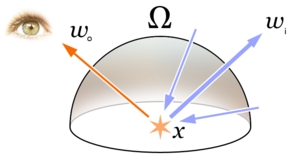
\includegraphics[scale=1.0]{rendering_eq.png}
\caption{Diagram representing the components of the rendering equation (image from \url{https://en.wikipedia.org/wiki/Rendering\_equation}).}
\label{fig:renderingeq}
\end{figure}

Of course, in order to compute this we must at the very least discretize the problem. Furthermore, the complexity involved in calculating all of the integrals that would be needed to render a full scene as stated by the rendering equation is computationally infeasible. Thus we need some way to approximate this complete model of light.

% TODO expand this, explain BRDF, Cook Torrance?

\section{Global Illumination}
To approximate the rendering equation it is helpful to divide light into two categories: direct and indirect light. Direct light for a point is calculated by iterating through all light sources in a scene and computing their contribution to the point. This is relatively easy and straightforward. Indirect lighting for a point is the light accumulated from non-light sources in the scene, like the ambient light that is bounced off of other surfaces.

The term global illumination generally refers to a lighting model which attempts to accurately approximate indirect illumination. Approaches like having a constant ambient light amount (as is done in the classic Phong~\cite{phong1975illumination} lighting model) and using ambient occlusion techniques like SSAO and HBAO do try to emulate some of the effects of indirect light but do not really attempt to accomplish full global illumination. For our algorithm, some of the main visual qualities we consider necessary are color bleeding and specular reflections (see Figure~\ref{fig:giqualities}). Here we give an overview of some techniques used to achieve more accurate global illumination.

\begin{figure}[h]
\centering
\makebox[\textwidth]{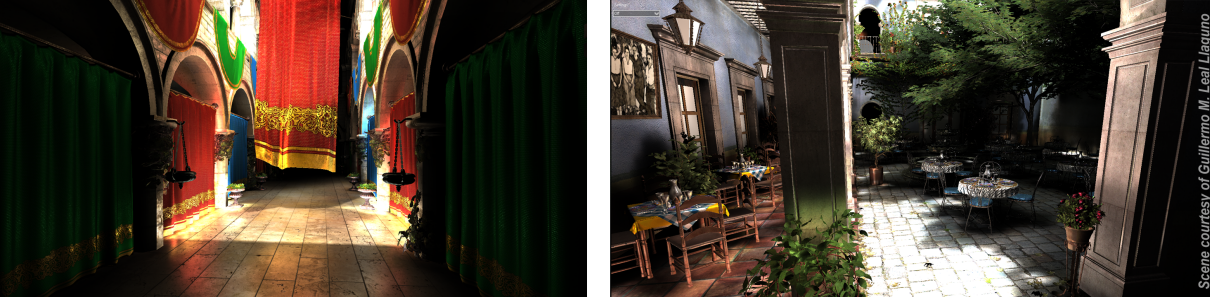
\includegraphics[width=\textwidth]{giqualities.png}}
\caption{Specular reflections can be seen on the ground of the left picture. Color bleeding can be seen on the archways of the left picture and on the column of the right picture. Images from~\cite{crassin2011interactive}.}
\label{fig:giqualities}
\end{figure}

% TODO raytracing and static lighting methods should probably be cut from background (not focus of this thesis, explain in intro)
\subsection{Monte Carlo Raytracing}
Raytracing is a common rendering technique which involves casting rays into a scene and determining color based on where the rays intersect. When a ray hits some geometry, direct lighting can be calculated by seeing if a ray from a light can `see' the intersection point. For indirect lighting, more work must be done. Monte Carlo Raytracing approximates the indirect light at a point by directly trying to approximate the surface integral over a hemisphere (as done in the rendering equation). This is done by only sending out a finite number of sampling rays to keep computation of the surface integral reasonable. The results, while impressive, still do not lend themselves well to real-time applications. Even with variations and improvements on the idea of raytracing, such as photon mapping, interactive frame rates are not achieved. 

\begin{figure}[h]
\centering
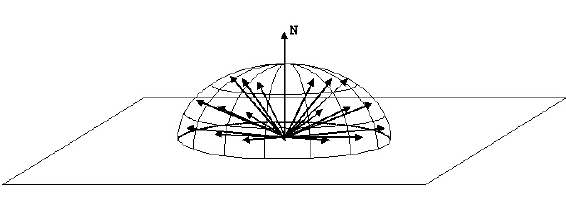
\includegraphics[scale=0.5]{sampling.png}
\caption{Sampling rays used to approximate an integral as would be done using Monte Carlo integration (image from \url{https://computergraphics.stackexchange.com/questions/4979}).}
\label{fig:sampling}
\end{figure}

\subsection{Baked Lighting}
Another approach to global illumination is to approximate the radiance in a scene using some spatial representation. Then, when computing the lighting the radiance can be looked up and used to achieve global illumination. Baked lighting follows this approach by pre-processing a scene's geometry and light sources in order to compute the radiance in a scene. During run time, the radiance can be looked up quickly. The clear and major drawback of this method is it is completely static: if a light or the geometry moves the radiance map created is no longer valid. Still, it is a great way to enhance visual quality when working with static lights and a relatively static scene.

\subsection{Voxel Cone Tracing}
The focus of much research, as well as this thesis, is on computing real-time global illumination with support for dynamic objects and lighting. Voxel cone tracing~\cite{crassin2011interactive} is a relatively recent method for computing this that has gained some popularity, with variations being implemented by NVIDIA~\cite{nvidiavxgi} (which is incorporated into the Unreal Engine) and some games~\cite{mclaren2016cascaded}.

The general voxel cone tracing algorithm relies on approximating the scene's radiance using a voxelized spatial data structure, which then upscales (filters) the radiance in order to obtain adequate performance. To perform the actual lighting calculation, the radiance is sampled from the spatial data structure in such a way to minimize the amount of sampling without sacrificing quality. More details on the basic voxel cone tracing algorithm will be provided in the Implementation chapter.
\fi
